\documentclass{report}

\usepackage{fullpage}
\usepackage{url}
\usepackage{amsthm}
\usepackage{amsmath}
\usepackage{amssymb}
\usepackage{cite}
\usepackage{listings}
\usepackage{graphicx}

\usepackage{tkz-graph}
\usetikzlibrary{arrows}
\usetikzlibrary{shapes}

\theoremstyle{plain}
\newtheorem{theorem}{Theorem}
\newtheorem{proposition}{Proposition}
\newtheorem{lemma}{Lemma}
\newtheorem*{corollary}{Corollary}

\theoremstyle{definition}
\newtheorem{definition}{Definition}
\newtheorem{conjecture}{Conjecture}
\newtheorem{example}{Example}
\newtheorem{algorithm}{Algorithm}

\theoremstyle{remark}
\newtheorem*{remark}{Remark}
\newtheorem*{note}{Note}
\newtheorem{case}{Case}

\numberwithin{definition}{chapter}
\numberwithin{example}{chapter}
\numberwithin{figure}{chapter}

\SetVertexNormal[Shape      = circle,
                 FillColor  = blue!20,
                 LineWidth  = 2pt]
\SetUpEdge[lw         = 2pt,
           color      = black,
           labelcolor = white,
           labeltext  = red,
           labelstyle = {sloped,draw,text=blue}]

\title{Parallelising graph algorithms in HPC-GAP \\ \vspace{2 mm} {\large University of St Andrews}}
\author{Ivars Zubkans \\ \small Supervised by: Dr James D Mitchell}

\begin{document}

\maketitle

\begin{abstract}

TODO - write an abstract probably something similar to the one below for CS.

The GAP system for computational discrete algebra did not have a general purpose package for graphs and graph theoretic algorithms. Moreover, parallelism capabilities were recently added in a high performance version of GAP. Therefore, this project implements a general purpose package for working with graphs. In addition, it is explored how the implemented algorithms can be modified to suit parallel execution. With the aim of having parallel implementations that scale with increase in number of processors and are faster than their serial counterparts, the parallel minimum spanning tree implementation partially scales with increase in number of processors and has a smaller scaling factor than its serial counterpart. The parallel breadth first search implementation did not scale very well with additional processors, but it is as fast as its serial counterpart for large graphs.
\end{abstract}

\tableofcontents

\chapter{Introduction}

TODO - the same as in CS at the moment, modify it at the end to reflect maths stuff covered.

Efficient implementations of graph theoretic algorithms are important due to their heavy use for modelling and solving problems in various fields. A graph represents connections between a set of objects. Thus graphs can be used to model relations in information, physical and social systems. Graph theory is used in areas of computer science such as data mining, image segmentation, clustering, image capturing and networking. Problems of efficiently planning network routes and diagnosing faults in computer networks are solved using graphs~\cite{6005872}. In chemistry and physics graphs are used to study molecules, atoms and construction of bonds. In biology graphs are used to model inhabitance regions of certain species and their migration paths. Similarly, graph theory is used in sociology to measure actors prestige or to explore diffusion mechanisms~\cite{shirinivas2010applications}. The aim of the project was to implements serial and parallel versions of graph algorithms in GAP and explore the possible performance gains of parallel implementations.

The GAP (\url{www.gap-system.org}) is a free open-source program for computing with various mathematical structures such as graphs, groups and fields. The graph related algorithms are in a package called Graph Algorithms Using Permutation Groups (GRAPE). This package is primarily used for working with graphs related to groups, finite geometries and designs. Thus it focuses on highly symmetric graphs to take advantage of the symmetries. There is no package for more standard graph algorithms such as traversal, path finding, minimum spanning tree algorithms and connected components in directed graphs.

Moreover, in a recent addition HPC-GAP supports both shared and distributed memory models. A shared memory can be used simultaneously by multiple programs to provide communication and remove redundancy. In a distributed memory each central unit of processing (CPU) has its own private memory. All of the current implementations in GRAPE are non-parallel.

Two GAP packages were made for serial and parallel implementations, so each made package is a self-contained extension to the core system of GAP. The serial package contains implementations of breadth first search, depth first search, vertex colouring using backtracking, Gabov's strongly connected components, Prim's minimum spanning tree and Dijkstra's shortest paths. The parallel implementation contains implementations for breadth first search, vertex colouring and finding minimum spanning trees under shared memory model. Then their performance was analysed and compared.

\section{Basic Graph Definitions}

A graph represents connections or relationships, called edges, between a set of elements, called vertices, more formally.

\begin{definition}[Graph]
A $graph$  $G$ is an ordered triple $G = (V, E, ends)$ where $V$ and $E$ are sets, while $ends$ is a function 
  \begin{equation}
  ends:E\to \mathcal P \left({V}\right)
  \end{equation}
which assigns to each element of $E$ a set of one or two elements of $V$. The elements of $V$ are called $vertices$ or $nodes$ of $G$, and elements of $E$ are called $edges$ of $G$ \cite{bondy2008graph}.
\end{definition}

The above definition is the one that will be used throughout the text instead of the most common graph definition:

\begin{definition}[Graph]
A $graph$  $G$ is an ordered pair of disjoint sets $G = (V, E)$ such that E is a subset of the set $V^{(2)}$ of unordered pairs of V, not necessarily distinct \cite{bollobas1998modern}. 
\end{definition} 

But in the second definition the edges between vertices are defined implicitly in terms of vertices and it is less clear that edges are separate objects that define the relationships between vertices. Therefore the first definition is used. Furthermore, the first definition includes the second, but the second definition does not. The second definition does not allow multiple edges between the same pair of vertices since in a set of edges there can be only one subset of the pair of vertices.

We will consider only $finite \ graphs$ - graphs with finite number of vertices and edges. Because the algorithmic problems and their considered solutions work in finite time only on finite graphs.

\begin{example}
An example of a graph is $G=(V, E, ends)$ where $V=\{1,2,3,4,5\}$, $E=\{\{1,2\}, \{2,3\}, \{3,1\}, \{4,3\}\}$ and is defined by the identity map, since $E \subseteq P(V)$. This illustrates how both graphs defined using the second definition could be defined using the first definition.

\begin{figure}[h]
\center
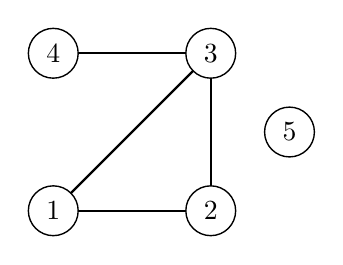
\begin{tikzpicture}
   \Vertex[x=0 ,y=0]{1}
   \Vertex[x=2,y=0]{2}
   \Vertex[x=2 ,y=2]{3}
   \Vertex[x=0 ,y=2]{4}
   \Vertex[x=3 ,y=1]{5}
   \Edge(1)(2)
   \Edge(2)(3)
   \Edge(3)(1)
   \Edge(3)(4)
\end{tikzpicture}
\caption{Graphical representation of a (simple, undirected) graph.}
\end{figure}
\end{example}

\begin{definition}[Incident]
Let $G = (V, E, ends)$ be a graph and $v\in V$ be a vertex, then v is $incident$ to an edge $e \in E$ if $v \in ends(e)$.
\end{definition}

\begin{definition}[Adjacent]
Let $G = (V, E, ends)$ be a graph and $v,w\in V$ be vertices, then $v$ and $w$ are adjacent if there is an edge $ e \in E$ such that $ends(e) = \{v, w\}$.
\end{definition}

\begin{definition}[Loop]
Let $G = (V, E, ends)$ be a graph and $e \in E$ be an edge , then $e$ is a $loop$ if $ends(e) = \{v\}$ for some vertex $v \in V$.
\end{definition}

\begin{definition}[Simple graph]
Let $G = (V, E, ends)$ be a graph, then $G$ is simple if
\begin{itemize}
\item $V$ is finite,
\item $G$ has no loops,
\item for any pair of vertices $v,w \in V$ there is at most one edge $e \in E$ such that $ends(e) = \{v, w\}$, i.e. there is at most one edge connecting a pair of vertices.
\end{itemize}
\end{definition}

We will generally consider simple graphs, but some of the implemented algorithms work on any graphs.

\begin{example}
The graph in the next example (figure \ref{loop}) has a loop at 4 and so is not simple. And for example the vertices 1 and 2 are adjacent, while 1 and 4 are not. Moreover, the edge between the vertices 1 and 2 is incident to 1 and 2.
\begin{figure}[h]
\center
\begin{tikzpicture}
   \Vertex[x=0 ,y=0]{1}
   \Vertex[x=2,y=0]{2}
   \Vertex[x=2 ,y=2]{3}
   \Vertex[x=0 ,y=2]{4}
   \Vertex[x=3 ,y=1]{5}
   \Edge(1)(2)
   \Edge(2)(3)
   \Edge(3)(1)
   \Edge(3)(4)
   \Loop[style={}](4)
\end{tikzpicture}
\caption{An example of graph with a loop}
\label{loop}
\end{figure}
\end{example}

\begin{definition}[Path]
Let $G = (V, E, ends)$ be a graph, then a $path$ in $G$ is a sequence $P$ of vertices $v_1,v_2,..,v_n$ such that $v_i$ and $v_{i+1}$ are adjacent for $1 \leq i \leq n - 1$, we say that $P$ is a path between $v_1$ and $v_n$.
\end{definition}

\begin{definition}[Connected]
Let $G = (V, E, ends)$ be a graph, then a $G$ is $connected$ if there exists a path between any pair of vertices in $V$ \cite{bollobas1998modern}.
\end{definition}

\begin{definition}[Subgraph]
Let $G = (V, E, ends)$ be a graph, then a subgraph of $G$ is a graph $G'=(V', E', ends')$ such that $V' \subseteq V$, $E' \subseteq E$ and $ends'$ is a restriction of $ends$ to $E'$ \cite{bondy2008graph}.
\end{definition}

\begin{definition}[Connected Component]
Let $G = (V, E, ends)$ be a graph, then a maximal connected subgraph of $G$ is called a $connected \ component$ \cite{bollobas1998modern}.
\end{definition}

Checking connectedness and finding connected components of a (undirected) graph is relatively easy, because in if there is a path from a vertex $v$ to a vertex $w$, then there is a path from $w$ to $v$, i.e. the connectedness is symmetric in (undirected) graphs. So connected components can be found by using BFS or DFS. Just pick a vertex and find all of its connected vertices using BFS or DFS. Repeat the process for vertices not yet in any component.

\section{Basic Algorithm Definitions}

\begin{definition}[Algorithm]
An $algorithm$ is a complete, step-by-step procedure for solving a specific problem in a finite amount of time. Each step has to be unambiguous and expressed in terms of finite number of rules \cite{berman1996fundamentals}.
\end{definition}

The rise of multi-processor and multi-core architectures has made the distinction between serial (sequential) and parallel algorithms an important one.

\begin{definition}[Serial Algorithm]
A $serial \ algorithm$ performs its steps in a sequence one at a time \cite{berman1996fundamentals}.
\end{definition}

\begin{definition}[Parallel Algorithm]
A $parallel \ algorithm$ performs many of its steps at the same time \cite{berman1996fundamentals}.
\end{definition}

We would like to compare different algorithms and analyse their theoretical performance without implementing them. Therefore we need to abstract away machine dependant details. The most common way of doing this is to use a hypothetical computer called $the Random Access Machine$. In Random Access machine every simple operation takes (arithmetic operations, branching, function calls) takes exactly one time step and loops are compositions of the simple operations. Furthermore, memory access takes exactly one time step, as caching is ignored and we assume to have enough random access memory \cite{skiena504algorithm}. Of course not all operations take exactly the same time, but this model is simple and captures the behaviour of a computer well enough. Therefore is used despite its limitations.

This model allows to count the number of steps an algorithm will take on a specific instance of a problem. So it only tells how good or bad and an algorithm is on a specific instance. Therefore we define worst-case, best-case and average-case complexities.

\begin{definition}[Worst-case complexity]
The $worst-case \ complexity$ of an algorithm is a function on natural numbers - the maximum number of steps taken by the algorithm on any instance of size n \cite{skiena504algorithm}.
\end{definition}

\begin{definition}[Average-case complexity]
The $average-case \ complexity$ of an algorithm is a function on natural numbers - the average number of steps taken by the algorithm on any instance of size n \cite{skiena504algorithm}.
\end{definition}

\begin{definition}[Best-case complexity]
The $best-case \ complexity$ of an algorithm is a function on natural numbers - the minimum number of steps taken by the algorithm on any instance of size n \cite{skiena504algorithm}.
\end{definition}

Best-case complexity is fairly useless in practice, because an algorithm could be really good on one instance (e.g. with a hard-coded solution), and really bad and take very long time on all other instances. Average-case complexity is hard to use, because 
We will use the worst-case complexity, because determining and characterising mathematically average inputs is difficult. Therefore we will generally use worst-case complexity.

Unfortunately these functions are often very complicated, therefore we will use their upper and lower bounds and discard their growth rates, because we mostly care how the algorithms scale anyway.

\begin{definition}[Upper bound]
A function $g(n)$ is an $upper \ bound$ of a function $f(n)$ if there exists some constant $c$ such that $f(n)\leq cg(n)$ always holds for large enough n. It is denoted by $f(n) = O(g(n))$ \cite{skiena504algorithm}.
\end{definition}

\begin{definition}[Lower bound]
A function $g(n)$ is an $lower \ bound$ of a function $f(n)$ if there exists some constant $c$ such that $f(n)\geq cg(n)$ always holds for large enough n. It is denoted by $f(n) = \Omega(g(n))$ \cite{skiena504algorithm}.
\end{definition}

\begin{definition}[Exact bound]
A function $g(n)$ is an $exact \ bound$ if it is both a lower and an upper bound (with possibly different constants) on another function $f(n)$, then it is denoted by $f(n) = \Theta(g(n))$
\end{definition}

We will generally try to find an upper bound, because the exact bound is usually harder to find and the lower bound is generally useless on its own. Note this ignores the constant growth factor of the complexity, i.e. functions $5n^2$ and $2n^2+1$ have the same lowest upper bound of $n^2$, therefore sometimes in practice one has to consider the growth factor at least for functions with the same lowest upper bound.

An algorithm is considered efficient time wise if its time complexity is $O(n)=log(n)$, because the logarithm function grows very slowly. Note that the logarithm base does not really matter, as it does not have a big impact on scaling. Although even polynomial time algorithms are considered good, especially when the polynomial is small. For parallel algorithms we strive to have a polylogarithmic worst-case complexity with a polynomial number of processors. Problems solvable by such algorithms are considered to be in the class called NC \cite{berman1996fundamentals}.

In this project we strived to implement algorithms that are correct, efficient both time and memory wise, while being easy to implement. Of course not always all three goals are achievable. Of course the most emphasis is placed on correctness, otherwise the implementations are useless. Therefore proofs of correctness are given. Note heuristics, algorithms giving approximate answers, are not considered in this project. Next we consider the efficiency the most important, because it allows to work with larger datasets faster without upgrading hardware. Despite that a balance is struck between efficiency and ease of implementation, as implementing very complicated algorithms is beyond the scope of this project. Efficiency wise bigger impact was placed on time complexity than space complexity, since machines with many processors generally have a lot of available memory.

Parallel algorithms have issues and constraints only specific to them \cite{berman1996fundamentals}:

\begin{itemize}
  \item Single instruction versus multiple instruction architecture. In a single instruction architecture only the same instruction can be executed in parallel, but possibly on different date. While in multiple instruction architecture does not have such a limitation. GAP follows multiple instruction architecture.
  \item Number and type of processors available. Parallel architectures have processors of varying capabilities. In GAP it is assumed that all processors are powerful enough to execute all normal instructions of a serial machine.
  \item Shared versus distributed memory model. GAP supports both, but we will use shared memory model, as it is easier to work with.
  \item Read and write restrictions. In GAP standard techniques of read and write locks and atomic objects are used to control concurrent access to the shared memory.
\end{itemize}

Thus designing and implementing parallel algorithms is generally harder. Therefore a number of approaches are used when designing parallel algorithms \cite{berman1996fundamentals}:
\begin{itemize}
  \item Modify an existing sequential algorithm exploiting those parts of the algorithm that are easily paralllizable. This approach is used to tackle vertex colouring.
  \item Come up with a completely new approach that may have not natural sequential analogue algorithm or it is not used for serial implementations. Naive algorithms are sometimes better suited for parallelism as they have more redundancy and are not squeezing everything out of the problem. This approach is used for finding the strongly connected components.
  \item For some problems just execute the same algorithm with different starting conditions on many processors until one finds a solution or the whole search space is covered.
\end{itemize}

\section{Implemented Algorithms}
\begin{itemize}
  \item Breadth first search
  \item Depth first search
  \item Strongly connected components
  \item Vertex colouring
  \item Minimum spanning trees
  \item Single source shortest paths
\end{itemize}

These algorithms were picked, because they are some of the most common graph algorithms that solve the most common graph problems. The other popular graph problems are travelling salesman problem, graph isomorphism and clique problem. Furthermore, they cover a wide range of different graphs (directed, undirected, weighted) and a range of different time complexities from linear to exponential. Note in this paper we describe only the strongly connected components, vertex colouring and single source shortest paths. For reference to other algorithms implemented see the computer science parts paper that is attached.

\chapter{Strongly Connected Components}

\section{Defining strongly connected components}

As discussed edges in a graph represent relationships between vertices. Often these are not symmetric and are represented using directed graphs, where edges have direction, i.e. there is a start and end vertex for each vertex.

\begin{definition}[Directed graph]
A $directed \ graph$  $G$ is a triple $G = (V, E, ends)$ where $V$ and $E$ are sets, while $ends$ is a function 
  \begin{equation}
  ends:E\to V \times V
  \end{equation}
which assigns to each element of $E$ a pair of two (possibly equal) elements of $V$ .
\end{definition}

\begin{definition}[Incident From]
Let $G = (V, E, ends)$ be a directed graph and $v \in V$ be a vertex, then $v$ is $incident \ From$ an edge $e \in E$ if $ends(e)=(v, w)$ for some vertex $w$.
\end{definition}

\begin{definition}[Incident To]
Let $G = (V, E, ends)$ be a directed graph and $v \in V$ be a vertex, then v is $incident \ to$ an edge $e \in E$ if $ends(e)=(w, v)$ for some vertex $w$.
\end{definition}

\begin{definition}[Adjacent To]
Let $G = (V, E, ends)$ be a directed graph and $v,w\in V$ be vertices, then $v$ is $adjacent \ to$ $w$ if there is an edge $ e \in E$ such that $ends(e) = \{v, w\}$.
\end{definition}

\begin{example}
An example of a directed graph is $G=(V, E, ends)$ where $V=\{1,2,3,4,5\}$, $E=\{(1,2), (2,3), (3,1), (4,3)\}$ and is defined by the identity map, since $E \subseteq V^2$. Moreover, 1 is adjacent to 2, edge (1,2) is incident from 1 and indecent to 2.

\begin{figure}[h]
\center
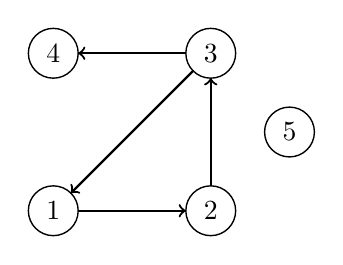
\begin{tikzpicture}
   \Vertex[x=0 ,y=0]{1}
   \Vertex[x=2,y=0]{2}
   \Vertex[x=2 ,y=2]{3}
   \Vertex[x=0 ,y=2]{4}
   \Vertex[x=3 ,y=1]{5}
   \tikzset{EdgeStyle/.style={->}}
   \Edge(1)(2)
   \Edge(2)(3)
   \Edge(3)(1)
   \Edge(3)(4)
\end{tikzpicture}
\caption{Graphical representation of a (simple) directed graph.}
\end{figure}
\end{example}

Now while checking connectedness and finding connected components is relatively easy in undirected graphs. It gets a bit more complicated for directed graphs, because there is not structural symmetry any more for categorizing connectedness. First, we need to distinguish between two different types of connectedness in directed graphs, because there are two directions for paths now - "forwards" and "backwards".

\begin{definition}[Strongly Connected]
Let $G = (V, E, ends)$ be a directed graph, then two vertices $v, w \in V$ of $G$ are $strongly \ connected$ if there exists a path from $v$ to $w$ and there exists a path from $w$ to $v$.
\end{definition}

\begin{definition}[Weakly Connected]
Let $G = (V, E, ends)$ be a directed graph, then two vertices $v, w \in V$ of $G$ are $weakly \ connected$ if either there exists a path from $v$ to $w$ or there exists a path from $w$ to $v$.
\end{definition}

Now we can define strongly connected components.

\begin{definition}[Strongly Connected Component]
Let $G = (V, E, ends)$ be a graph, then a maximal strongly connected subgraph of $G$ is called a $strongly \ connected \ component$ of $G$.
\end{definition}

\begin{example}
An example of strongly connected components of a directed graph. The components are subgraphs induced by vertices $\{1,6,3,4\}$, $\{2,7,8\}$, $\{5\}$ and $\{9\}$.

\begin{figure}[h]
\center
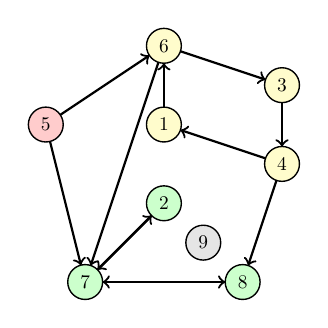
\begin{tikzpicture}[scale=0.5]
   \tikzset{EdgeStyle/.style={->}}
   \tikzset{VertexStyle/.append  style={fill=yellow!20, scale=0.7]}}
   \Vertex[x=0 ,y=0]{1}
   \tikzset{VertexStyle/.append  style={fill=yellow!20}}
   \Vertex[x=3,y=1]{3}
   \Vertex[x=3 ,y=-1]{4}
   \Vertex[x=0 ,y=2]{6}
   \tikzset{VertexStyle/.append  style={fill=green!20}}
   \Vertex[x=0 ,y=-2]{2}
   \Vertex[x=-2 ,y=-4]{7}
   \Vertex[x=2 ,y=-4]{8}
   \tikzset{VertexStyle/.append  style={fill=red!20}}
   \Vertex[x=-3 ,y=0]{5}
   \tikzset{VertexStyle/.append  style={fill=gray!20}}
   \Vertex[x=1 ,y=-3]{9}
   \Edge(6)(3)
   \Edge(3)(4)
   \Edge(4)(1)
   \Edge(1)(6)
   \Edge(4)(8)
   \Edge(6)(7)
   \Edge(2)(7)
   \Edge(7)(2)
   \Edge(7)(8)
   \Edge(8)(7)
   \Edge(5)(6)
   \Edge(5)(7)
\end{tikzpicture}
\caption{Strongly connected components of a directed graph}
\end{figure}
\label{SCC_example}
\end{example}

Now that we have defined strongly connected components, the goal of a strongly connected components algorithm is to partition the vertices $V$ of a directed graph $G=(V,E,ends)$ into strongly connected components. It is usually done by assigning component index numbers to each vertex, either starting from zero or $|V|$ (1 or $|V|+1$ for 1-index based programming languages), this also allows to easily determine the number of strongly connected components.

\section{Serial algorithms}

The very simplest approach to find strongly connected components is brute force algorithm. Using DFS or BFS check for every pair of two vertices $v$ and $w$ that there is a path from $v$ to $w$ and from $w$ to $v$, i.e. just run BFS or DFS on $v$ and then on $w$ until $w$ and $v$ is found, respectively. Of course this algorithm is very inefficient. Its time complexity is $O(V^2E)$ (for a strongly connected graph). It is because we are repeating almost the same search for every pair of vertices in the same strongly connected component. Therefore we can do much better. As we will see later, strongly connected components can be found in linear time, i.e. its time complexity is $O(V + E)$.

The three most common algorithms for finding strongly connected components are Kosaraju's, Tarjan's and Gabow's algorithms. Moreover all three have linear time and space complexity \cite{c++_sedgewick}. Kosaraju's algorithm works by running DFS with postordering on the reverse (direction of edges is reversed) of the graph and then running a second DFS. After an iteration of the second DFS is exhausted. The next iteration of the second DFS is started at a yet unvisited vertex with the highest postorder number given by the first DFS \cite{c++_sedgewick}. The Tarjan's algorithm is based on DFS and uses a stack to keep track of the current search path. A sequence of vertices is only popped from the top of the stack when it is determined that all of them are in the same strongly connected component. It happens when the last vertex of the strongly connected component is visited and can be determined by maintaining the lowest index  reachable vertex for each vertex \cite{c++_sedgewick}. The Gabow's algorithm is very similar except that a second stack is used to maintain the lowest reachable vertex \cite{c++_sedgewick}.

Tarjan's and Gabov's algorithms are preferable over Kosaraju's, because they pass through the graph only once and do not require a computation of the reverse graph \cite{c++_sedgewick}. The performance of Tarjan's and Gabov's algorithms is essentially the same, since they are very similar. The performance differences are likely to be small or platform-dependent \cite{Gabow2000107}. So the choice between them is fairly arbitrary. Therefore Gabov's algorithm was picked, as I found it a little bit easier to implement.

\subsection{Gabow's algorithm}

This subsection is based on the Gabow's original paper \cite{Gabow2000107} on his algorithm.

\subsubsection*{High Level algorithm}

Let $G=(V, E, ends)$ be a directed graph, then we can form another graph - the graph $H$ of strongly connected components of $G$ formed by contracting the vertices of each strongly connected component. So strongly connected components of $H$ are single vertices. This graph is acyclic (has no cycles), since all vertices in a cycle are strongly connected, but no vertices in $H$ are strongly connected. This leads us to a high level algorithm proposed by Purdom and Munro.

The algorithm builds the graph $H$ by contracting $G$ and maintaining a path $P$ in $H$. Initially $H=G$. If $H$ has no vertices stop, as there are no strongly connected components then. Otherwise start a new path $P$ by picking a vertex $v$ and setting $P = (v)$ Then grow $P=(v_1,v_2,...,v_k)$ by choosing an unprocessed vertex $w$ adjacent to $v_k$ and doing as follows:

\begin{itemize}
  \item If $w \not \in P$, then add $w$ to $P$ and keep growing $P$.
  \item If $w \in P$ say $w=v_i$, then contract the cycle $v_i,v_{i+1},...,v_k$ to $w$ both in $H$ and in $P$ and keep growing $P$.
  \item If $v_k$ after all contractions has no unprocessed adjacent vertices left, remove $v_k$ from $P$ and keep it as a vertex of the strongly connected components graph - final version of $H$. Now if $P \not = \emptyset$, keep growing $P$. Otherwise pick another not contracted vertex in $H$ and start a new path $P$.
\end{itemize}

This algorithm builds $H$, because all cycles are contracted and the last vertex $v_k$ of $P$ vertex is kept in $H$ only when all vertices reachable from it are processed. Thus the algorithm correctly computes the strongly connected components.

\begin{example}

An example of executing the high level algorithm on the graph $G$ in example \ref{SCC_example} to find its strongly connected components graph. The first contracted cycle is $(1,6,3,4)$, the next is $(7,2)$ and then $(8,7)$. The vertices of each contracted cycle are in the same strongly connected component, so in the end vertex $1$ represents strongly connected component with vertices $1,6,3,4$ and $8$ with $8,7,2$. Thus this gives us all 4 strongly connected components of $G$.

\begin{figure}[h]
\center

\begin{minipage}[h]{0.24\textwidth}
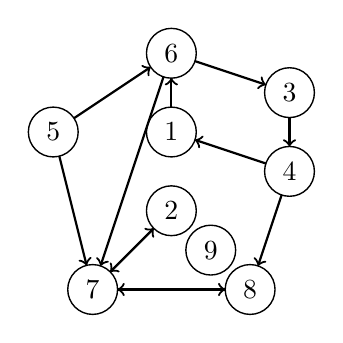
\begin{tikzpicture}[scale=0.5]
   \tikzset{EdgeStyle/.style={->}}
   \Vertex[x=0 ,y=0]{1}
   \Vertex[x=3,y=1]{3}
   \Vertex[x=3 ,y=-1]{4}
   \Vertex[x=0 ,y=2]{6}
   \Vertex[x=0 ,y=-2]{2}
   \Vertex[x=-2 ,y=-4]{7}
   \Vertex[x=2 ,y=-4]{8}
   \Vertex[x=-3 ,y=0]{5}
   \Vertex[x=1 ,y=-3]{9}
   \Edge(6)(3)
   \Edge(3)(4)
   \Edge(4)(1)
   \Edge(1)(6)
   \Edge(4)(8)
   \Edge(6)(7)
   \Edge(2)(7)
   \Edge(7)(2)
   \Edge(7)(8)
   \Edge(8)(7)
   \Edge(5)(6)
   \Edge(5)(7)
\end{tikzpicture}

Initially $H=G$
\end{minipage}
\hfill
\minipage{0.24\textwidth}
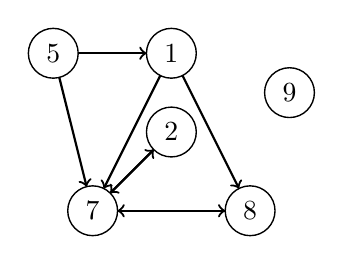
\begin{tikzpicture}[scale=0.5]
   \tikzset{EdgeStyle/.style={->}}
   \Vertex[x=0 ,y=0]{1}
   \Vertex[x=0 ,y=-2]{2}
   \Vertex[x=-2 ,y=-4]{7}
   \Vertex[x=2 ,y=-4]{8}
   \Vertex[x=-3 ,y=0]{5}
   \Vertex[x=3 ,y=-1]{9}
   \Edge(1)(8)
   \Edge(1)(7)
   \Edge(2)(7)
   \Edge(7)(2)
   \Edge(7)(8)
   \Edge(8)(7)
   \Edge(5)(1)
   \Edge(5)(7)
\end{tikzpicture}

After first contraction

when $P=(1,6,3,4)$

and $w=1$
\endminipage\hfill
\minipage{0.24\textwidth}
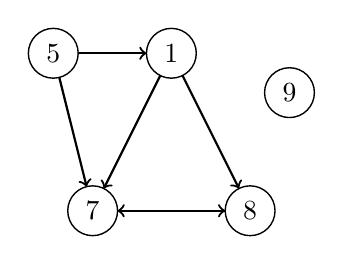
\begin{tikzpicture}[scale=0.5]
   \tikzset{EdgeStyle/.style={->}}
   \Vertex[x=0 ,y=0]{1}
   \Vertex[x=-2 ,y=-4]{7}
   \Vertex[x=2 ,y=-4]{8}
   \Vertex[x=-3 ,y=0]{5}
   \Vertex[x=3 ,y=-1]{9}
   \Edge(1)(8)
   \Edge(1)(7)
   \Edge(7)(8)
   \Edge(8)(7)
   \Edge(5)(1)
   \Edge(5)(7)
\end{tikzpicture}

After second contraction

when $P=(1,8,7,2)$

and $w=7$
\endminipage\hfill
\minipage{0.24\textwidth}
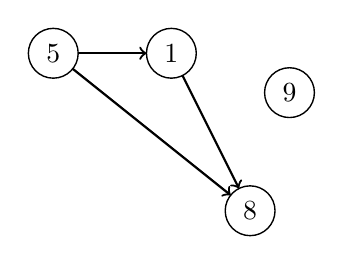
\begin{tikzpicture}[scale=0.5]
   \tikzset{EdgeStyle/.style={->}}
   \Vertex[x=0 ,y=0]{1}
   \Vertex[x=2 ,y=-4]{8}
   \Vertex[x=-3 ,y=0]{5}
   \Vertex[x=3 ,y=-1]{9}
   \Edge(1)(8)
   \Edge(5)(1)
   \Edge(5)(8)
\end{tikzpicture}

After third contraction

when $P=(1,8,7)$

and $w=8$
\endminipage\hfill

\caption{Example of finding the strongly connected components graph}
\end{figure}
\label{high_example}
\end{example}

\subsubsection*{Gabow's implementation}

Now the implementations of the high level algorithm by Purdom and Munro were not efficient. Therefore Tarjan's algorithm was used instead. But then Gabow found an efficient linear time implementation of the high level algorithm using only two stacks $S$ and $B$ and DFS. The stack $S$ contains the original sequence of vertices in $P$ as visited by DFS, i.e. the whole path without removing contracted vertices. While the stack $B$ contains the boundaries between contracted vertices, i.e. the positions of vertices in S that are left in $P$ after contraction. So if $P=(v_1, v_2,...v_k)$ then $k$ is at the top of $B$ and for all $i = 1,...k-1$ we have $v_i=\{ S[j] : B[i] \leq j < B[i+1] \}$, i.e. the vertex $v_i$ represents all contracted vertices that are strongly connected.

We assume all $n=|V|$ vertices of $G$ are indexed from $1$ to $n$. In addition to stacks $S$ and $B$ an array/list $I[1..n]$ stores position in the stack $S$ for each vertex or the index of the strongly connected component it belongs to.  More specifically for a vertex $v$, $I[v] = 0$ if $v$ has not been in $P$ yet, $I[v]=j$ for some integer $j$ if $v$ is currently in $P$ and $S[j]=v$, finally $I[v]=c$ if the strongly connected component of $v$ has been completed and its index is $c$. Note we assign indices larger than $n$ to strongly connected components, so there is no confusion between vertex's stack position $j$ in $S$ and component index $c$.

Now the algorithm performs DFS of the given graph $G$, while maintaining $S$, $B$ and $I$. When a vertex $v$ is visited by DFS it is pushed onto $S$ and its position in $S$ is pushed onto $B$. Because clearly $v$ now is on the path $P$ and is not (yet) strongly connected with the previously visited vertex as this is the first time visiting $v$. Therefore its position (boundary) is pushed onto $B$.

When a vertex $w$ that is already visited is discovered again by DFS, say $P=v_1,v_2,...v_k$ and $w=v_i$. Then we have found a cycle. Therefore all the vertices $v_{i+1},...v_k$ visited after $w$ and $w$ are strongly connected. So we contract them to a single vertex $v_i=\{ S[j] : B[i] \leq j < B[i+1] \}$. To do that pop off positions (boundaries) of all vertices after $w$ by just popping them of until $B[top(b)] \leq I[w]$. Thus only boundaries vertex positions in $S$ from a found strongly connected component are maintained on $B$.

After processing all the edges for each vertex $v$ and returning from recursive calls, we check if a vertex's $v$ position is at the top of the stack $B$. If it is we have found a complete strongly connected component. It consists of $v$ and all vertices on $S$ after $v$. Because we have found all reachable vertices from $v$ and all the vertices left on $S$ are strongly connected to $v$, since its position is at the top of $B$. So we just pop all the vertices before $v$ from S and add them to a new strongly connected component. Once this modified DFS is finished we have found all strongly connected components of $G$ and each vertex $v$ of $G$ is assigned its strongly connected components index.

\subsubsection*{Pseudo-code}

\begin{lstlisting}[language=Ruby]
def SCC(G)

S1:  Create an empty stack S
S2:  Create an empty stack B
S3:  Create a list I marking all vertices as unvisited

S4:  for each yet undiscovered vertex v
S5:    SCC_DFS(G, v)
end

def SCC_DFS(G, v)
  
D1:  Push v onto S
D2:  Push top(S) on B
  
D3:  for each vertex w adjacent to v
D4:    if w is not discovered
D5:      SCC_DFS(G, w)
D6:    else
         # Pop all positions of vertices discovered after w from B
D7:      while I[w] < B[top(B)] do
D8:        pop(B)
  
       # if position of v in S is at top of B
D9:    if I[v] = B[top(B)]
D11      pop(B)
D12:     Pop all vertices w after v from S
D13:     Mark all w as in the same strongly connected component as v
end
\end{lstlisting}

\begin{example}

An example of executing the Gabow's algorithm on the graph $G$ in example \ref{SCC_example} to find its strongly connected components. The state of $S$, $B$ and $I$ is given at the same moments as in example \ref{high_example} and at the moments when  
returning from recursive call for a vertex $v$ its position is at the top of the stack $B$. Note processing of vertices 5 and 9 ends almost immediately, as they have only outgoing edges or no edges at all, respectively. Thus their steps are combined in the example.

\begin{figure}[h]

\begin{minipage}[h]{0.24\textwidth}
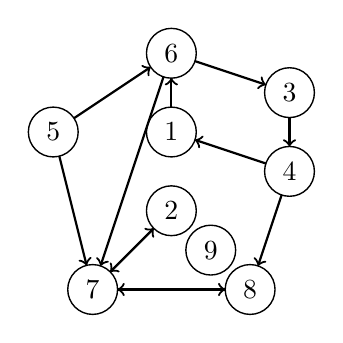
\begin{tikzpicture}[scale=0.5]
   \tikzset{EdgeStyle/.style={->}}
   \Vertex[x=0 ,y=0]{1}
   \Vertex[x=3,y=1]{3}
   \Vertex[x=3 ,y=-1]{4}
   \Vertex[x=0 ,y=2]{6}
   \Vertex[x=0 ,y=-2]{2}
   \Vertex[x=-2 ,y=-4]{7}
   \Vertex[x=2 ,y=-4]{8}
   \Vertex[x=-3 ,y=0]{5}
   \Vertex[x=1 ,y=-3]{9}
   \Edge(6)(3)
   \Edge(3)(4)
   \Edge(4)(1)
   \Edge(1)(6)
   \Edge(4)(8)
   \Edge(6)(7)
   \Edge(2)(7)
   \Edge(7)(2)
   \Edge(7)(8)
   \Edge(8)(7)
   \Edge(5)(6)
   \Edge(5)(7)
\end{tikzpicture}

$I=[0, 0, 0, 0, 0, 0, 0, 0, 0]$

$S=[]$

$B=[]$

\end{minipage}
\hfill
\minipage{0.24\textwidth}
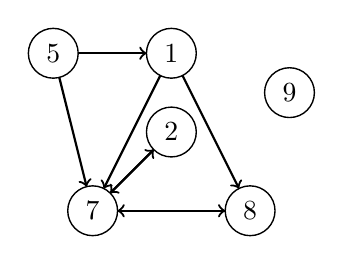
\begin{tikzpicture}[scale=0.5]
   \tikzset{EdgeStyle/.style={->}}
   \Vertex[x=0 ,y=0]{1}
   \Vertex[x=0 ,y=-2]{2}
   \Vertex[x=-2 ,y=-4]{7}
   \Vertex[x=2 ,y=-4]{8}
   \Vertex[x=-3 ,y=0]{5}
   \Vertex[x=3 ,y=-1]{9}
   \Edge(1)(8)
   \Edge(1)(7)
   \Edge(2)(7)
   \Edge(7)(2)
   \Edge(7)(8)
   \Edge(8)(7)
   \Edge(5)(1)
   \Edge(5)(7)
\end{tikzpicture}

After first contraction,

when $P=(1,6,3,4)$

and $w=1$,

$I=[1, 0, 3, 4, 0, 2, 0, 0, 0]$

$S=[1, 3, 4, 6]$

B=[1, 2, 3, 4] to B=[1]
\endminipage\hfill
\minipage{0.26\textwidth}
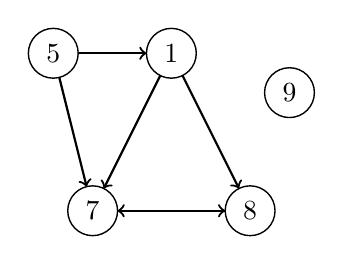
\begin{tikzpicture}[scale=0.5]
   \tikzset{EdgeStyle/.style={->}}
   \Vertex[x=0 ,y=0]{1}
   \Vertex[x=-2 ,y=-4]{7}
   \Vertex[x=2 ,y=-4]{8}
   \Vertex[x=-3 ,y=0]{5}
   \Vertex[x=3 ,y=-1]{9}
   \Edge(1)(8)
   \Edge(1)(7)
   \Edge(7)(8)
   \Edge(8)(7)
   \Edge(5)(1)
   \Edge(5)(7)
\end{tikzpicture}

After second contraction,

when $P=(1,8,7,2)$

and $w=7$,

$I=[1, 7, 3, 4, 0, 2, 6, 5, 0]$

$S=[1, 3, 4, 6, 8, 7, 2]$

B=[1, 5, 6, 7] to B=[1, 5, 6]
\endminipage\hfill
\minipage{0.24\textwidth}
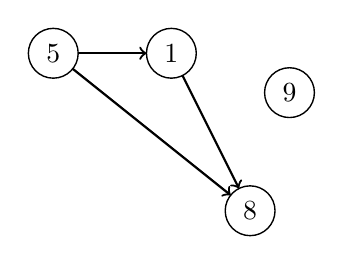
\begin{tikzpicture}[scale=0.5]
   \tikzset{EdgeStyle/.style={->}}
   \Vertex[x=0 ,y=0]{1}
   \Vertex[x=2 ,y=-4]{8}
   \Vertex[x=-3 ,y=0]{5}
   \Vertex[x=3 ,y=-1]{9}
   \Edge(1)(8)
   \Edge(5)(1)
   \Edge(5)(8)
\end{tikzpicture}

After third contraction,

when $P=(1,8,7)$

and $w=8$,

$I=[1, 7, 3, 4, 0, 2, 6, 5, 0]$

$S=[1, 3, 4, 6, 8, 7, 2]$

$B=[1, 5, 6]$ to $B=[1, 5]$
\endminipage\hfill

\vspace*{2\baselineskip}

\minipage{0.33\textwidth}
After done with vertex 8:

$I=[1, 10, 3, 4, 0, 2, 10, 10, 0]$

$S=[1, 3, 4, 6]$

$B=[1]$
\endminipage\hfill
\minipage{0.33\textwidth}
After done with vertex 1:

$I=[11, 10, 11, 11, 0, 11, 10, 10, 0]$

$S=[]$

$B=[]$
\endminipage\hfill
\minipage{0.33\textwidth}
End after processing 5 and then 9:

$I=[11, 10, 11, 11, 12, 11, 10, 10, 13]$

S=[5] to S=[] to S=[9] to S=[]

B=[1] to B=[] to B=[1] to B=[]
\endminipage\hfill


\caption{Example of finding the strongly connected components of a graph using Gabow's algorithm}
\end{figure}
\end{example}

\begin{theorem}
Gabow's algorithm finds the strongly connected components of a directed graph $G=(V,E,ends)$ in linear time and space.
\end{theorem}

\begin{proof}
We will prove the first part of the theorem by proving that Gabow's algorithm is a valid implementation of the high level algorithm.
An implementation of the high level algorithm must specify how a path $P=(v_1,v_2,...,v_k)$ is grown. More specifically how it chooses an unprocessed vertex $w$ adjacent to $v_k$ to grow $P$. When $w$ is added to $P$ as the last new vertex, we say that $w$ is activated. Moreover we say that the most active vertex is the currently activated vertex, i.e we order active vertices in their order of activation. Now to choose the next unprocessed vertex $w$ adjacent to $v_k$, let $v$ be the most active vertex. If there is an unprocessed vertex $w$ adjacent to $v$ pick it. If $v$ does not have any unprocessed adjacent vertices left, then deactivate $v$. If this makes all vertices of $v_k$ inactive, then make a strongly connected component from all vertices of $v_k$ and remove it from $P$. This correctly implements the high-level algorithm, because the most active vertex $v$ always belongs to the last vertex $v_k$ of $P$. Notice the activation mechanism mimics recursive DFS.

Now we need to prove that SCC implements the above version of the high level algorithm. We do this by the number of executed statements in SCC, i.e. the number of DFS iterations. If there are no vertices and thus no DFS iterations, the algorithm just returns an empty list, which is correct since there are no strongly connected components in an empty graph. Now assume the algorithm works for $k$ iterations and we must check it for $k+1$ iterations.

When we call SCC\_DFS in line S5 after $k$ iterations, by the inductive assumption for all unvisited vertices $u$ we have $I[u]=0$ and for all visited vertices $z$ we have $I[z] > n$, since we have found and completed all strongly connected components for all vertices. Moreover $P$ and thus $S$ and $B$ are empty, as we are just starting a new path. During the loop at D3 (excluding recursion), $v$ is the most active vertex, since we have just added it to $P$ or deactivated vertices after $v$. In D4 a vertex $w$ is not yet visited, if $I[w]=0$. If $0 < I[w] \leq n$, let $i=I[w]$  then D5 contracts a cycle $(S[i],S[i+1],...S[top(S)])$ or does nothing if it is already contracted, because it pops off positions of all vertices after $w$ by just popping them of until $B[top(b)] \leq I[w]$. If $I[w] > n$ then the component containing $w$ has been deleted and D5 again does nothing.

At D9 we have processed all adjacent vertices to $v$ and check if vertex's $v$ position is at the top of the stack $B$. If it is we have found a complete strongly connected component. It consists of $v$ and all vertices on $S$ after $v$. Because we have found all reachable vertices from $v$ and all the vertices left on $S$ are strongly connected to $v$, since we have contracted all vertices on $P$ after $v$ in some combinations of cycles and removed the rest of them that are not those cycles by completing their strongly connected components beforehand. So after processing the initial vertex we assigned component indices to all visited vertices and have emptied $P$, $S$ and $B$ again. This completes the proof  of the first part of the theorem.

Proving second part of the theorem is relatively straightforward. If the given graph $G$ is stored using adjacency lists. Note that every vertex is pushed (when visited) and popped (when added to a strongly connected component or when contracted) from each stack S and B exactly once and every edge is examined exactly once, too. Thus the algorithm spends constant time and space for each vertex or edge. Therefore it is linear in time and space.
\end{proof}

\chapter{Vertex colouring}

\chapter{shortest paths}

\bibliographystyle{plain}
\bibliography{References}
\end{document}